\documentclass{beamer}
\usepackage[outputdir=build]{minted}
\usepackage[skins,minted,breakable]{tcolorbox}
\usepackage[spanish]{babel}
\usepackage{subcaption}
\usepackage{multicol}
\graphicspath{ {../img/} {../../LaTeX/img/} {/home/csp98/latex/img/}}
\selectlanguage{spanish}
\newtheorem{ppio_invarianza}{Principio de Invarianza}
\usepackage[utf8]{inputenc}
\usetheme{PaloAlto}
\setbeamerfont{section in sidebar}{size=\fontsize{2}{4}\selectfont}
\setbeamerfont{subsection in sidebar}{size=\fontsize{2}{3}\selectfont}
\setbeamerfont{subsubsection in sidebar}{size=\fontsize{2}{2}\selectfont}

\setbeamerfont{section in toc}{size=\footnotesize}
\setbeamerfont{subsection in toc}{size=\scriptsize}
\setbeamerfont{subsubsection in toc}{size=\tiny}




\title{Práctica 1}

\subtitle{Análisis de eficiencia de algoritmos}

\author{María Jesús López Salmerón \\ Nazaret Román Guerrero \\ Laura Hernández Muñoz \\ José Baena Cobos  \\ Carlos Sánchez Páez}

\makeatletter
  \setbeamertemplate{sidebar \beamer@sidebarside}%{sidebar theme}
  {
    \beamer@tempdim=\beamer@sidebarwidth%
    \advance\beamer@tempdim by -6pt%
    \insertverticalnavigation{\beamer@sidebarwidth}%
    \vfill
    \ifx\beamer@sidebarside\beamer@lefttext%
    \else%
      \usebeamercolor{normal text}%
      \llap{\usebeamertemplate***{navigation symbols}\hskip0.1cm}%
      \vskip2pt%
    \fi%
}%
\makeatother

\subject{Algorítmica}

\AtBeginSubsection[]
{
  \begin{frame}<beamer>{Índice}
    \tableofcontents[currentsection,currentsubsection]
  \end{frame}
}

% Let's get started
\begin{document}

\begin{frame}
  \titlepage
\end{frame}

\begin{frame}{Índice}
  \tableofcontents
  % You might wish to add the option [pausesections]
\end{frame}


\section{Cálculo de la eficiencia empírica}

\subsection{Diseño de scripts}

\begin{frame}[fragile]{Script individual}
\begin{minted}[fontsize=\small]{bash}
	#!/bin/bash
	if [ $# -eq 3 ] then;
		i="0"
		output="out"
		tam=$2
		#Primer argumento: programa a ejecutar
		#Segundo argumento: tamaño inicial
		#Tercer argumento : incremento
		while [ $i -lt 25 ]
		do
			./$1 $tam >> $1.out
			i=$[$i+1]
			tam=$[$tam+$3]
		done
	else
		echo "Error de argumentos"
	fi
\end{minted}  
\end{frame}

\begin{frame}[fragile]{Script conjunto}

\begin{minted}[fontsize=\small]{bash}
	#!/bin/bash
	echo "Ejecutando burbuja..."
	./individual.sh burbuja 1000 1000
	echo "Ejecutando insercion..."
	./individual.sh insercion 1000 1000
	echo "Ejecutando seleccion..."
	./individual.sh seleccion 1000 1000
	echo "Ejecutando mergesort..."
	./individual.sh mergesort 1000000 500000
	echo "Ejecutando quicksort..."
	./individual.sh quicksort 1000000 500000
	echo "Ejecutando heapsort..."
	./individual.sh heapsort 1000000 500000
	echo "Ejecutando hanoi..."
	./individual.sh hanoi 10 1
	echo "Ejecutando floyd..."
	./individual.sh floyd 100 100
\end{minted}  
\end{frame}

\begin{frame}[fragile]{Makefile}

\begin{minted}[fontsize=\tiny]{makefile}
	DOC=doc
	SRC=src
	OUT=out
	BIN=src

	all : todos
	todos : burbuja floyd hanoi heapsort insercion mergesort quicksort seleccion
		cd $(SRC) ; ./todos.sh
	burbuja : 
		g++ -o ./$(BIN)/burbuja ./$(SRC)/burbuja.cpp
	floyd : 
		g++ -o ./$(BIN)/floyd ./$(SRC)/floyd.cpp
	hanoi : 
		g++ -o ./$(BIN)/hanoi ./$(SRC)/hanoi.cpp
	heapsort : 
		g++ -o ./$(BIN)/heapsort ./$(SRC)/heapsort.cpp
	insercion : 
		g++ -o ./$(BIN)/insercion ./$(SRC)/insercion.cpp
	mergesort : 
		g++ -o ./$(BIN)/mergesort ./$(SRC)/mergesort.cpp
	quicksort : 
		g++ -o ./$(BIN)/quicksort ./$(SRC)/quicksort.cpp
	seleccion :
		g++ -o ./$(BIN)/seleccion ./$(SRC)/seleccion.cpp
\end{minted}  
\end{frame}

\begin{frame}[fragile]{Generación de gráficas}

\begin{minted}[fontsize=\small]{bash}

	#!/usr/bin/gnuplot
	set xlabel "Tamanio del problema"
	set ylabel "Tiempo (seg)"
	set terminal png size 640,480
	
	#Burbuja
	set output 'empirica_burbuja.png'
	plot 'burbuja.out' with lines

	#Floyd
	set output 'empirica_floyd.png'
	plot 'floyd.out' with lines

	#Hanoi
	set output 'empirica_hanoi.png'
	plot 'hanoi.out' with lines
				...
\end{minted}
\end{frame}

\subsection{Modificación de código fuente}

\begin{frame}[fragile]{Modificación de código fuente}
\begin{minted}{c++}
	clock_t tantes;
	clock_t tdespues;
	tantes = clock();
	algoritmo_en_cuestion(T, n);
	tdespues = clock();
	cout << ((double)(tdespues - tantes))
	/ CLOCKS_PER_SEC << endl;
\end{minted}
\end{frame}


\subsection{Tamaños de problema}
\begin{frame}[fragile]{Tamaños de problema}
\begin{table}[H]
\centering
\resizebox{\textwidth}{!}{%
\begin{tabular}{|c|c|c|c|c|}
\hline
\textbf{Algoritmo} & \textbf{Eficiencia} & \textbf{Tamaño inicial} & \textbf{Tamaño final} & \textbf{Incremento}\\
\hline
Burbuja &  &  &  &  \\
Inserción & $O(n^2)$ & 1000 & 25000 & 1000 \\
Selección &  &  & &  \\
\hline
Mergesort & & & & \\
Quicksort & $O(n \cdot log(n))$ & 1.000.000 & 13.000.000 & 500.000 \\
Heapsort &  & & &  \\
\hline
Floyd & $O(n^3)$ & 100 & 2500 & 100 \\
\hline
Hanoi & $O(2^n)$ & 10 & 34 & 1 \\
\hline
\end{tabular}
}
\end{table}
\end{frame}
\subsection{Resultados}

\subsubsection{Algoritmos con eficiencia $O(n^2)$}

\begin{frame}[fragile]{Algoritmo burbuja}
\begin{figure}[H]
\centering
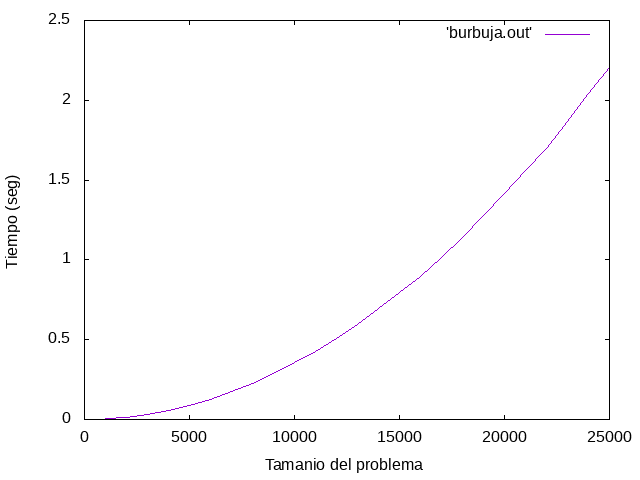
\includegraphics[scale=0.5]{empirica_burbuja.png}
\end{figure}
\end{frame}

\begin{frame}[fragile]{Algoritmo de inserción}
\begin{figure}[H]
\centering
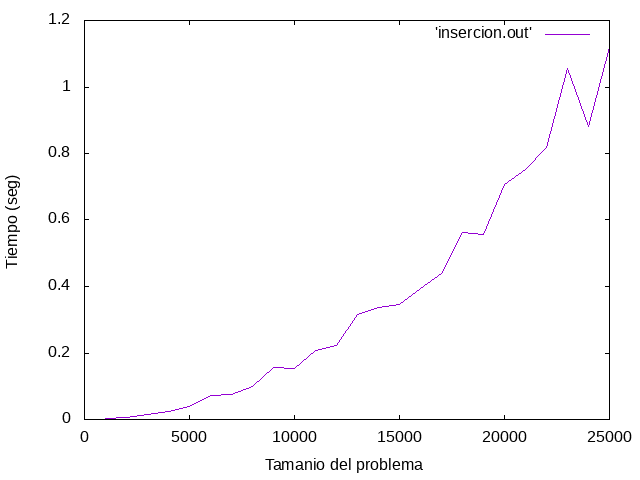
\includegraphics[scale=0.5]{empirica_insercion.png}
\end{figure}
\end{frame}

\begin{frame}[fragile]{Algoritmo de selección}
\begin{figure}[H]
\centering
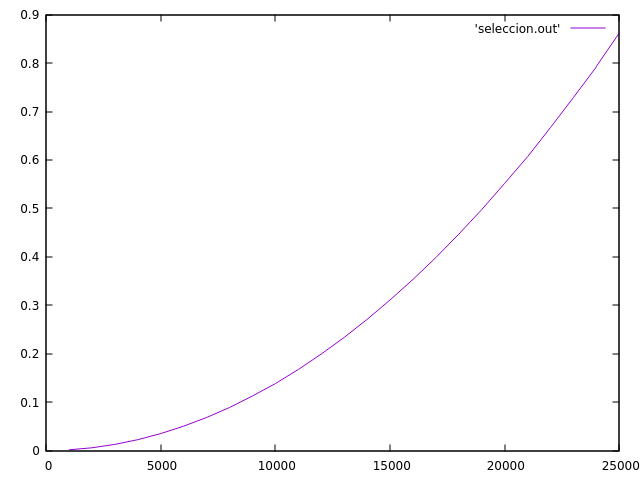
\includegraphics[scale=0.5]{empirica_seleccion.png}
\end{figure}
\end{frame}

\subsubsection{Algoritmo con eficiencia $O(n^3)$}
\begin{frame}[fragile]{Algoritmo de Floyd}
\begin{figure}[H]
\centering
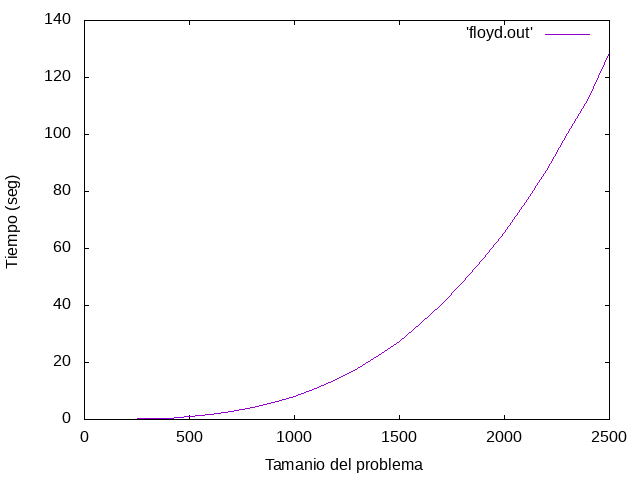
\includegraphics[scale=0.5]{empirica_floyd.png}
\end{figure}
\end{frame}

\subsubsection{Algoritmos con eficiencia $O(n \cdot log(n))$}

\begin{frame}[fragile]{Algoritmo mergesort}
\begin{figure}[H]
\centering
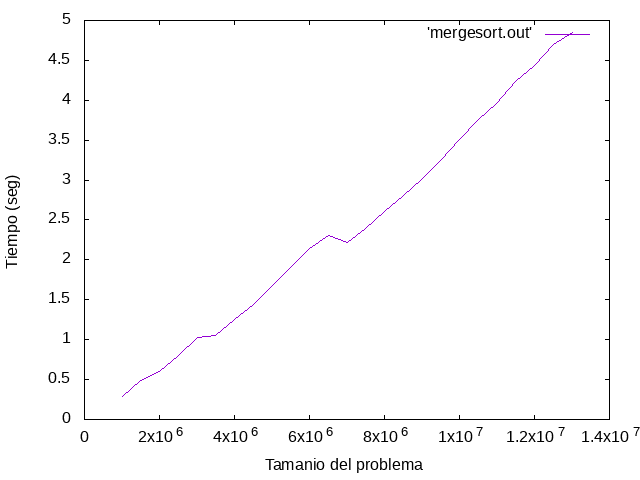
\includegraphics[scale=0.5]{empirica_mergesort.png}
\end{figure}
\end{frame}

\begin{frame}[fragile]{Algoritmo quicksort}
\begin{figure}[H]
\centering
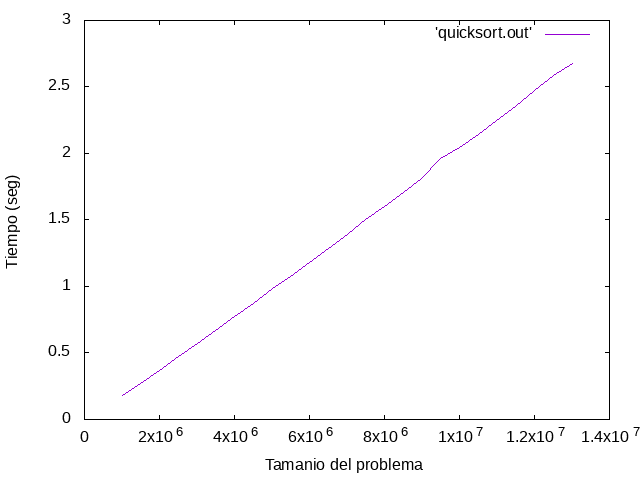
\includegraphics[scale=0.5]{empirica_quicksort.png}
\end{figure}
\end{frame}

\begin{frame}[fragile]{Algoritmo heapsort}
\begin{figure}[H]
\centering
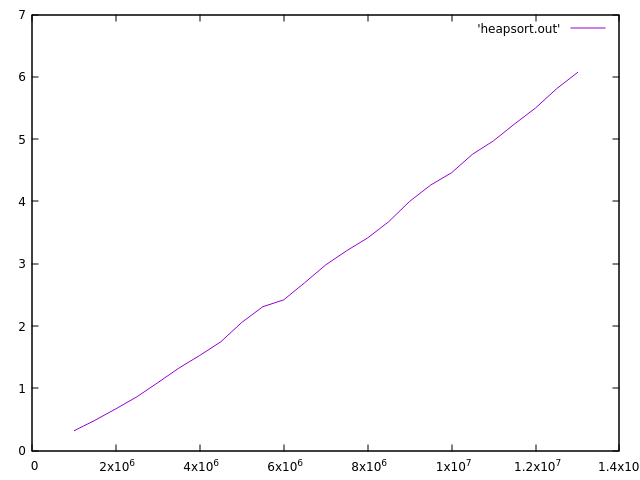
\includegraphics[scale=0.5]{empirica_heapsort.png}
\end{figure}
\end{frame}

\subsubsection{Algoritmo con eficiencia $O(2^n)$}

\begin{frame}[fragile]{Algoritmo Hanoi}
\begin{figure}[H]
\centering
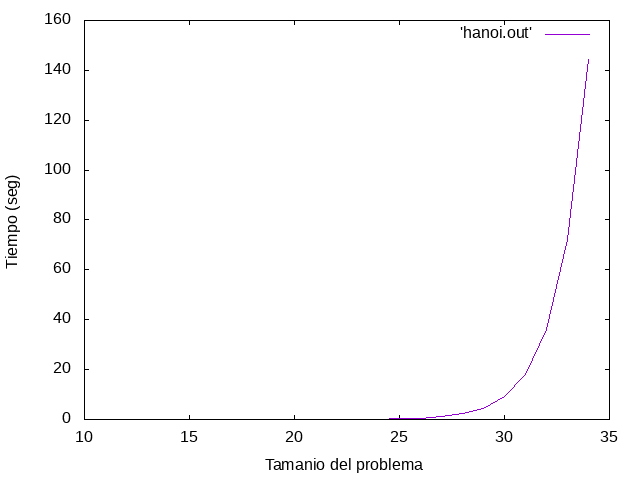
\includegraphics[scale=0.5]{empirica_hanoi.png}
\end{figure}
\end{frame}

\subsection{Entornos de pruebas}
\begin{frame}[fragile]{Comparación de entornos}
\begin{table}[H]
\centering
\resizebox{\textwidth}{!}{%
\begin{tabular}{|c|c|c|c|}
\hline
\textbf{Componente} & \textbf{Característica} & \textbf{PC 1} & \textbf{PC 2}\\
\hline
 & Modelo & AMD FX-8320 @3.5Ghz & Intel Core i7-6700HQ @2.60Ghz \\

 & Frecuencia máxima & 4.20Ghz & 3.5Ghz \\
CPU & Caché L1 & 16K(i)+64K(d)  & 32K(i)+32K(d) \\
 & Caché L2 & 2048K & 256K \\
 & Caché L3 & 8192K & 6144K \\
\hline
 & Capacidad & 16384MB & 8192MB \\
RAM & Frecuencia & 1600Mhz & 2133Mhz \\
 & Tecnología & DDR3 & DDR4 \\
\hline
\end{tabular}
}
\end{table}
\end{frame}

\subsection{Variación de la eficiencia empírica}
\begin{frame}[fragile]{Variación de la eficiencia empírica}
\begin{ppio_invarianza}
La eficiencia empírica varía al cambiar de plataforma, lenguaje, etc. como mucho en una constante.
\end{ppio_invarianza}
\end{frame}

\begin{frame}[fragile]{Tiempos de ejecución en cada plataforma}
\begin{table}[H]
\centering
\resizebox{\textwidth}{!}{%
\begin{tabular}{|c|c|c|c|}
\hline
\textbf{Algoritmo} & \textbf{Tiempo medio PC 1} & \textbf{Tiempo medio PC 2} & \textbf{Constante} \\
\hline
Burbuja & 0,366 & 0,251 & 1,456\\
\hline
Inserción & 0,172 & 0,100 & 1,715\\
\hline
\textit{Selección} & 0,144 & 0,124 & 1,159\\
\hline
\textit{Mergesort} & 1,948 & 1,422 & 1,371\\
\hline
\textit{Quicksort} & 1,144 & 0,965 & 1,186\\
\hline
\textit{Heapsort} & 2,314 & 1,821 & 1,271\\
\hline
Floyd & 8,636 & 5,348 & 1,615\\
\hline
Hanoi & 0,036 & 0,023 & 1,538\\
\hline
\end{tabular}
}
\end{table}
\end{frame}


\subsubsection{Algoritmos con eficiencia $O(n^2)$}

\begin{frame}[fragile]{Algoritmo burbuja}
\begin{figure}[H]
\centering
\begin{minipage}{.5\textwidth}
  \centering
  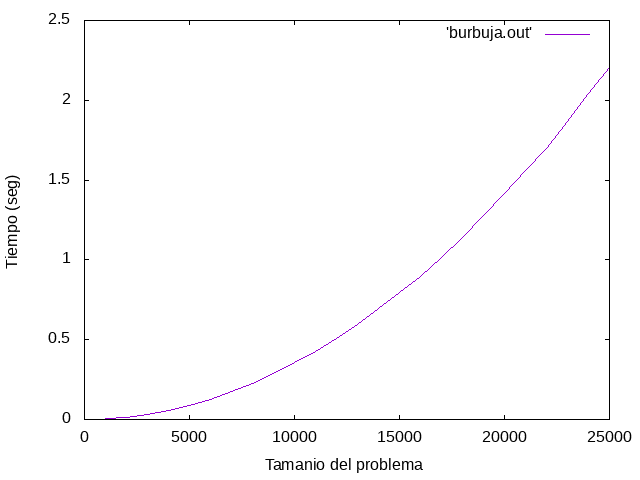
\includegraphics[width=\linewidth]{empirica_burbuja.png}
   \caption*{PC 1}
\end{minipage}%
\begin{minipage}{.5\textwidth}
  \centering
  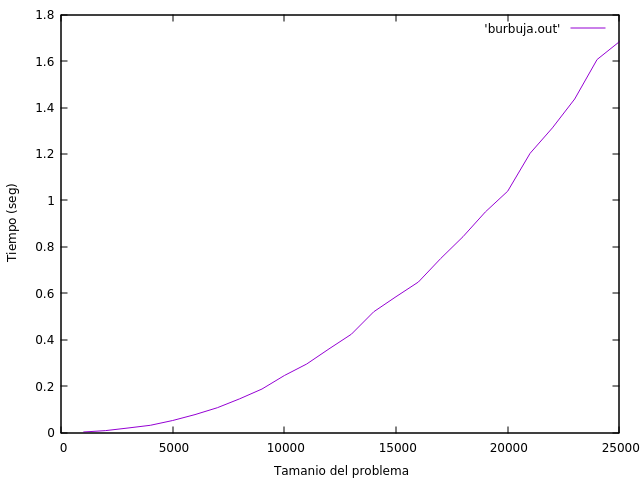
\includegraphics[width=\linewidth]{empirica_burbuja_2.png}
  \caption*{PC 2}
\end{minipage}
\end{figure}
\end{frame}

\begin{frame}[fragile]{Algoritmo de inserción}
\begin{figure}[H]
\centering
\begin{minipage}{.5\textwidth}
  \centering
  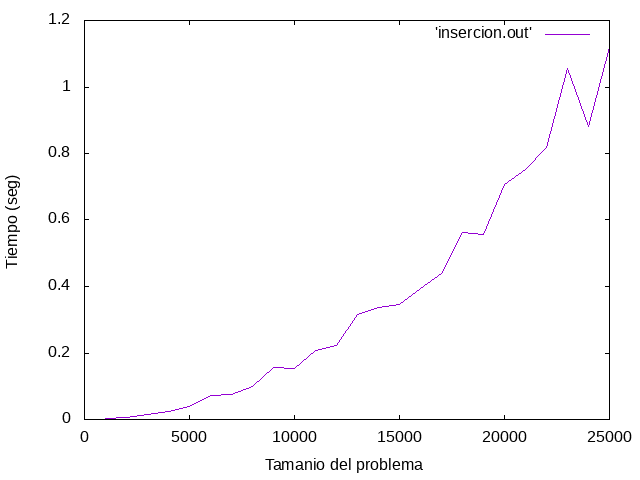
\includegraphics[width=\linewidth]{empirica_insercion.png}
   \caption*{PC 1}
\end{minipage}%
\begin{minipage}{.5\textwidth}
  \centering
  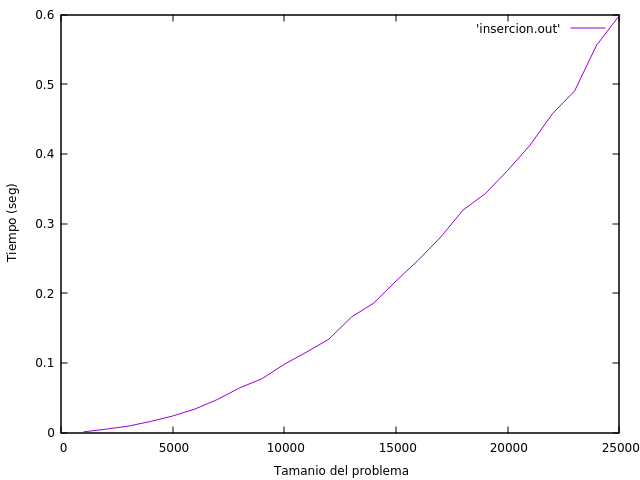
\includegraphics[width=\linewidth]{empirica_insercion_2.png}
  \caption*{PC 2}
\end{minipage}
\end{figure}
\end{frame}

\begin{frame}[fragile]{Algoritmo de selección}
\begin{figure}[H]
\centering
\begin{minipage}{.5\textwidth}
  \centering
  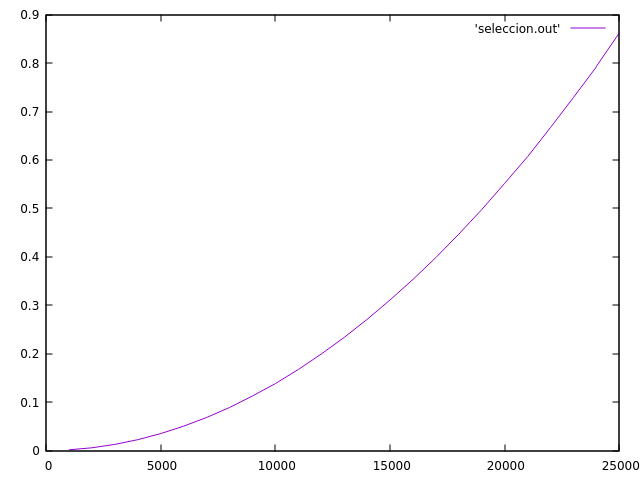
\includegraphics[width=\linewidth]{empirica_seleccion.png}
   \caption*{PC 1}
\end{minipage}%
\begin{minipage}{.5\textwidth}
  \centering
  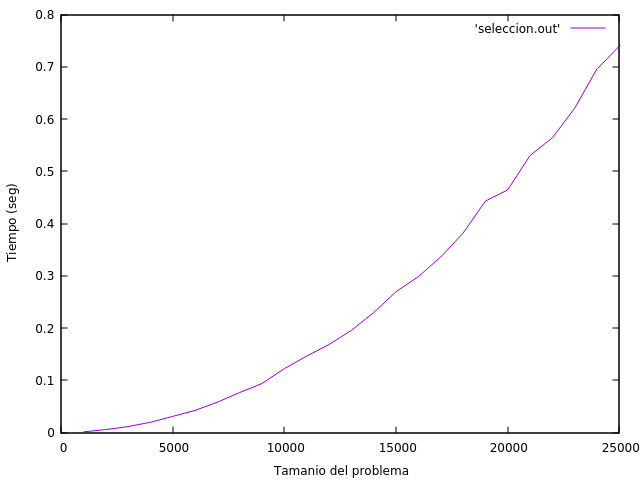
\includegraphics[width=\linewidth]{empirica_seleccion_2.png}
  \caption*{PC 2}
\end{minipage}
\end{figure}
\end{frame}

\subsubsection{Algoritmo con eficiencia $O(n^3)$}
\begin{frame}[fragile]{Algoritmo de Floyd}
\begin{figure}[H]
\centering
\begin{minipage}{.5\textwidth}
  \centering
  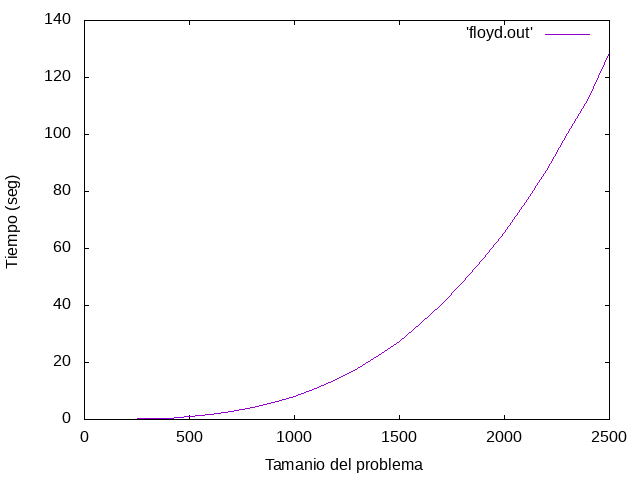
\includegraphics[width=\linewidth]{empirica_floyd.png}
   \caption*{PC 1}
\end{minipage}%
\begin{minipage}{.5\textwidth}
  \centering
  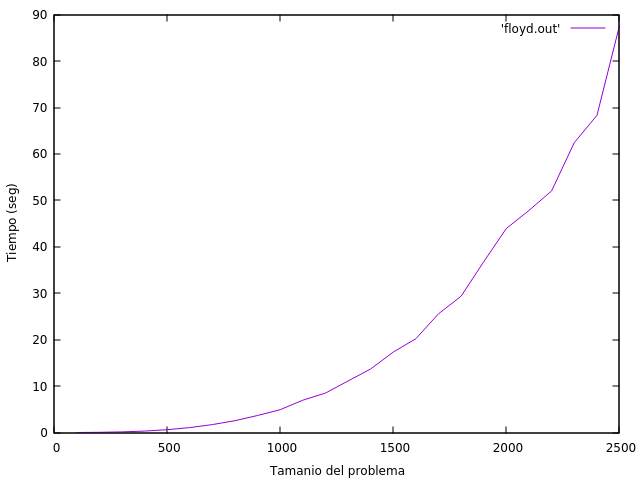
\includegraphics[width=\linewidth]{empirica_floyd_2.png}
  \caption*{PC 2}
\end{minipage}
\end{figure}
\end{frame}

\subsubsection{Algoritmos con eficiencia $O(n \cdot log(n))$}

\begin{frame}[fragile]{Algoritmo mergesort}
\begin{figure}[H]
\centering
\begin{minipage}{.5\textwidth}
  \centering
  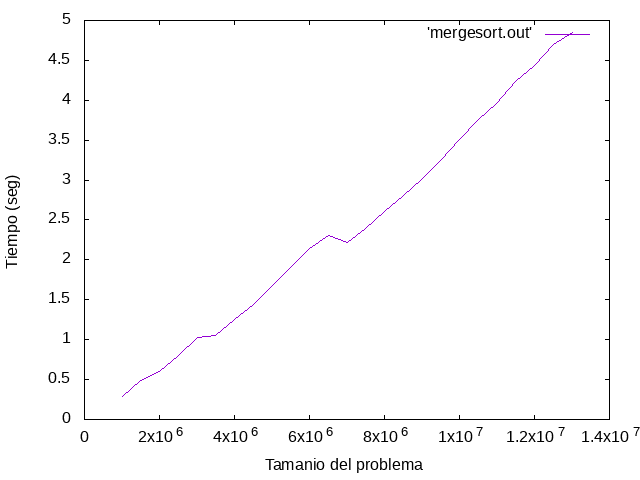
\includegraphics[width=\linewidth]{empirica_mergesort.png}
   \caption*{PC 1}
\end{minipage}%
\begin{minipage}{.5\textwidth}
  \centering
  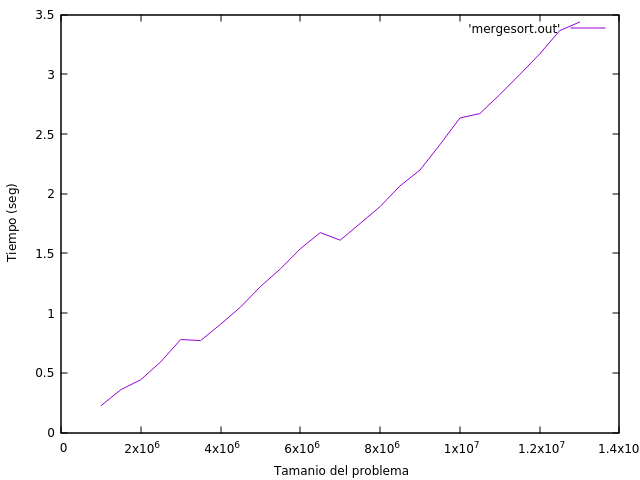
\includegraphics[width=\linewidth]{empirica_mergesort_2.png}
  \caption*{PC 2}
\end{minipage}
\end{figure}
\end{frame}

\begin{frame}[fragile]{Algoritmo quicksort}
\begin{figure}[H]
\centering
\begin{minipage}{.5\textwidth}
  \centering
  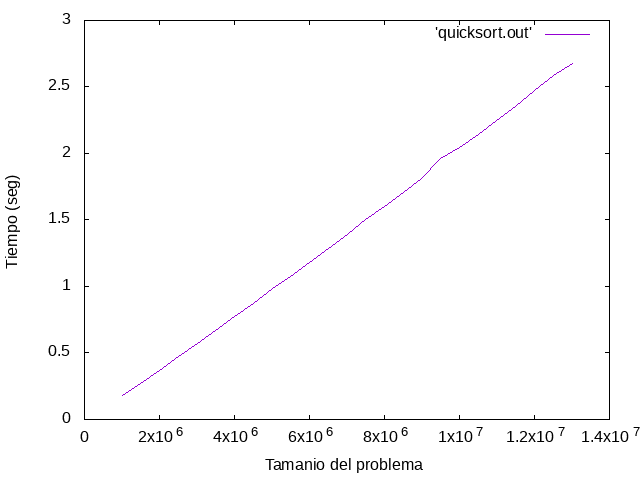
\includegraphics[width=\linewidth]{empirica_quicksort.png}
   \caption*{PC 1}
\end{minipage}%
\begin{minipage}{.5\textwidth}
  \centering
  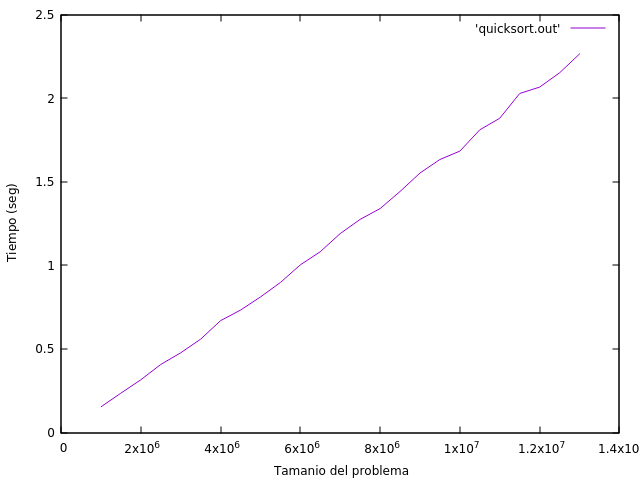
\includegraphics[width=\linewidth]{empirica_quicksort_2.png}
  \caption*{PC 2}
\end{minipage}
\end{figure}
\end{frame}

\begin{frame}[fragile]{Algoritmo heapsort}
\begin{figure}[H]
\centering
\begin{minipage}{.5\textwidth}
  \centering
  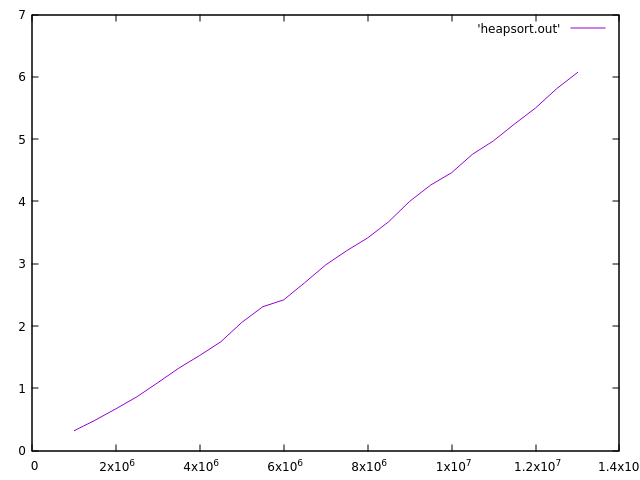
\includegraphics[width=\linewidth]{empirica_heapsort.png}
   \caption*{PC 1}
\end{minipage}%
\begin{minipage}{.5\textwidth}
  \centering
  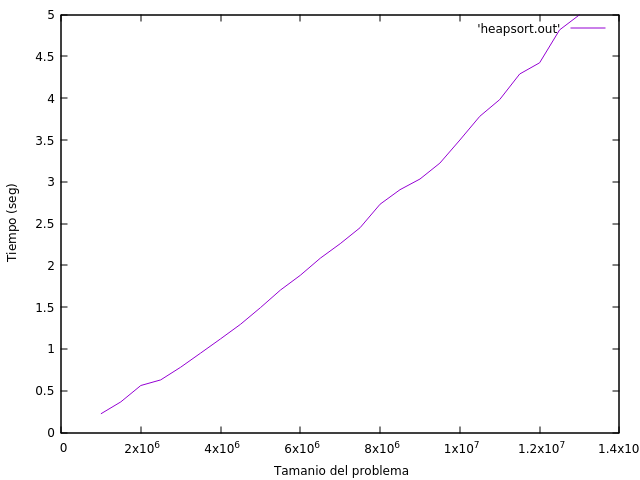
\includegraphics[width=\linewidth]{empirica_heapsort_2.png}
  \caption*{PC 2}
\end{minipage}
\end{figure}
\end{frame}

\subsubsection{Algoritmo con eficiencia $O(2^n)$}

\begin{frame}[fragile]{Algoritmo Hanoi}
\begin{figure}[H]
\centering
\begin{minipage}{.5\textwidth}
  \centering
  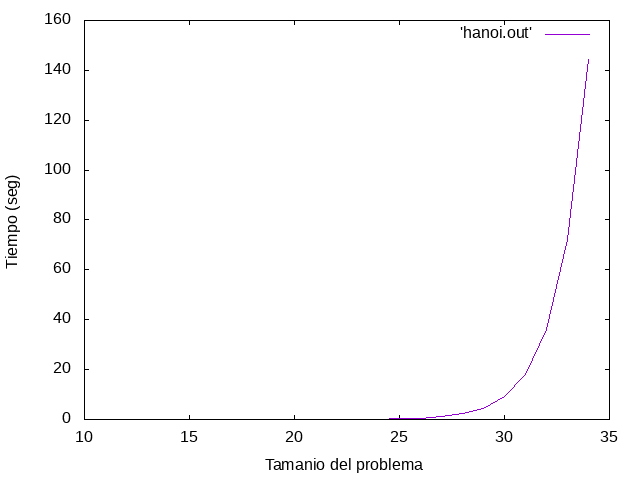
\includegraphics[width=\linewidth]{empirica_hanoi.png}
   \caption*{PC 1}
\end{minipage}%
\begin{minipage}{.5\textwidth}
  \centering
  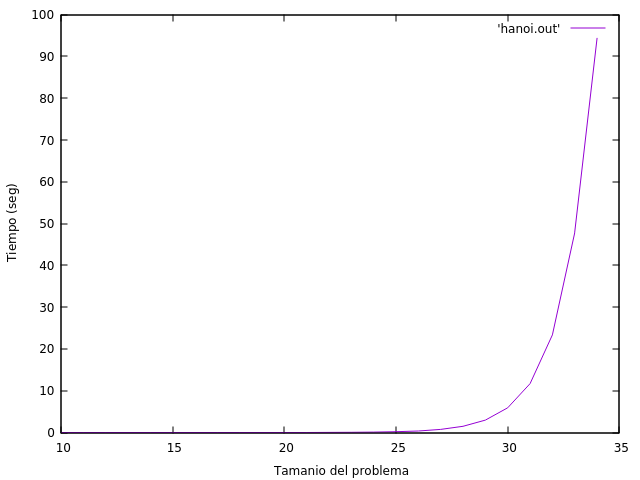
\includegraphics[width=\linewidth]{empirica_hanoi_2.png}
  \caption*{PC 2}
\end{minipage}
\end{figure}
\end{frame}
\subsection{Comparación de algoritmos}
\begin{frame}[fragile]{Comparación entre algoritmos}
\begin{figure}[H]
\centering
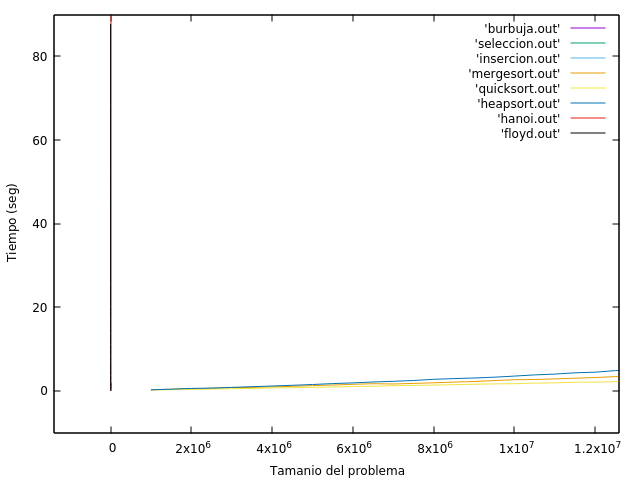
\includegraphics[scale=0.5]{empirica_todos.png}
\end{figure}
\end{frame}


\begin{frame}[fragile]{Comparación entre algoritmos (zoom)}
\begin{figure}[H]
\centering
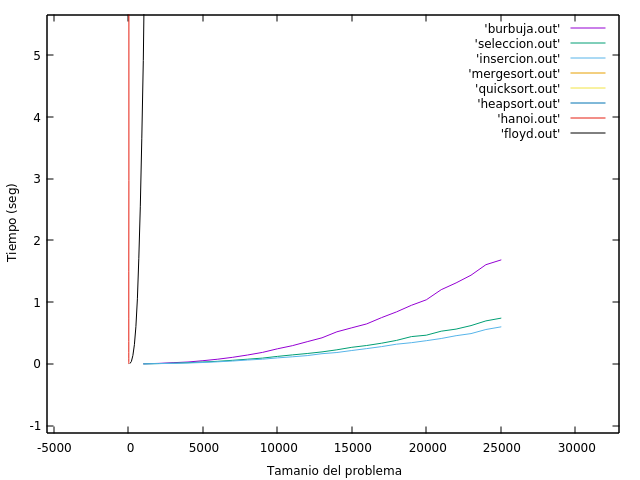
\includegraphics[scale=0.5]{empirica_todos_zoom.png}
\end{figure}
\end{frame}

\subsubsection{Comparación entre algoritmos de ordenación}

\begin{frame}[fragile]{Comparación entre algoritmos de ordenación}
\begin{figure}[H]
\centering
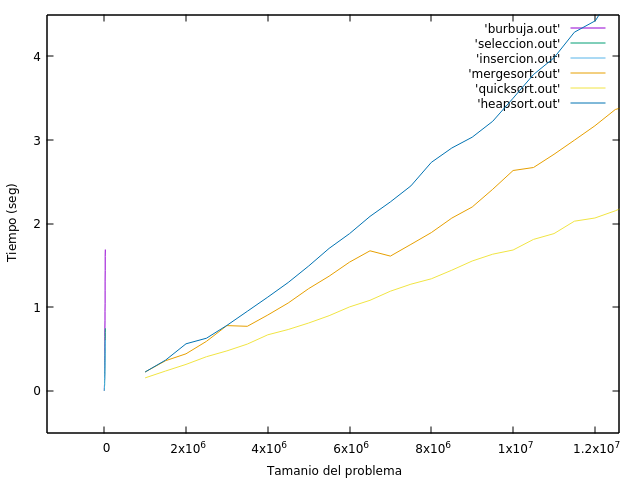
\includegraphics[scale=0.5]{empirica_ordenacion_comparacion.png}
\end{figure}
\end{frame}

\begin{frame}[fragile]{Comparación entre algoritmos de ordenación (zoom)}
\begin{figure}[H]
\centering
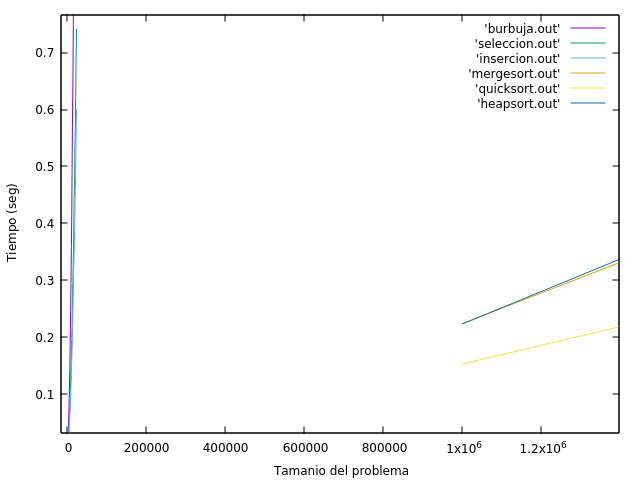
\includegraphics[scale=0.5]{empirica_ordenacion_comparacion_zoom.png}
\end{figure}
\end{frame}

\section{Cálculo de la eficiencia híbrida}

\subsection{Errores en el cálculo de la constante oculta}
\begin{frame}[fragile]{Errores en el cálculo de la constante oculta}
\begin{table}[H]
\centering
\resizebox{\textwidth}{!}{%
\begin{tabular}{|c|c|c|}
\hline
\textbf{Algoritmo} & \textbf{Orden de eficiencia} & \textbf{Porcentaje de error} \\
\hline
Burbuja &  & 2.253e-12 (0.06377\%)\\
Selección & $n^2$ & 3.047e-13 (0.02211\%)\\
Inserción & & 3.085e-11 (1.805\%) \\
\hline
Heapsort &  & 2.071e-10 (0.7626\%) \\
Mergesort & $n \cdot log(n)$ & 1.893e-10 (0.8614\%) \\
Quicksort & & 1.407e-11 (0.1113\%) \\
\hline
Hanoi & $2^n$ & 1.095e-12 (0.01302\%) \\
\hline
Floyd & $n^3$ & 7.291e-12 (0.08874\%) \\
\hline
{\color{red}Ajuste erróneo} & {\color{red}$2^n$ a $n^2$} & {\color{red}0.00868(26.86\%)}\\
\hline
\end{tabular}
}
\end{table}
\end{frame}

\subsection{Resultados}

\subsubsection{Algoritmos con eficiencia $O(n^2)$}

\begin{frame}[fragile]{Algoritmo burbuja}
\begin{figure}[H]
\centering
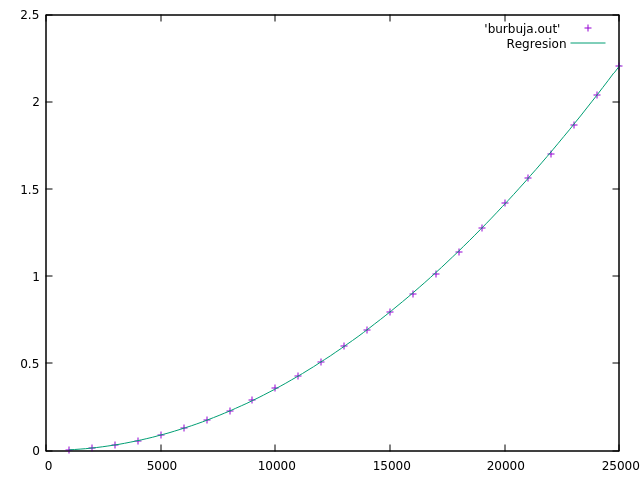
\includegraphics[scale=0.5]{hibrida_burbuja.png}
\end{figure}
\end{frame}

\begin{frame}[fragile]{Algoritmo de inserción}
\begin{figure}[H]
\centering
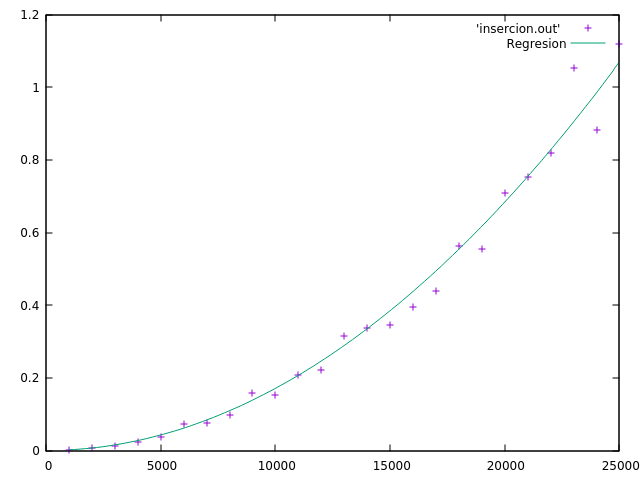
\includegraphics[scale=0.5]{hibrida_insercion.png}
\end{figure}
\end{frame}

\begin{frame}[fragile]{Algoritmo de selección}
\begin{figure}[H]
\centering
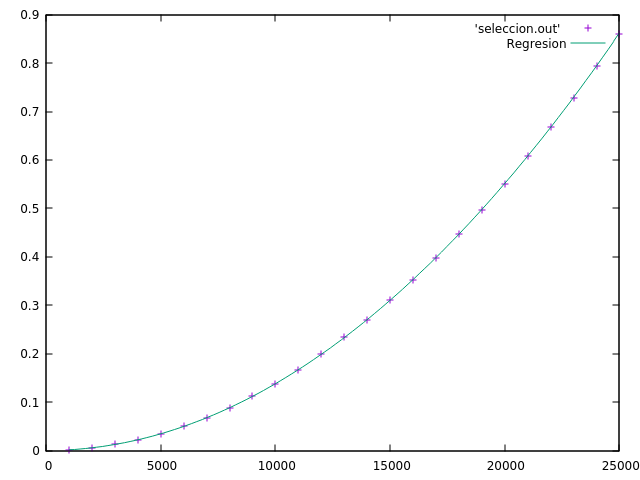
\includegraphics[scale=0.5]{hibrida_seleccion.png}
\end{figure}
\end{frame}

\subsubsection{Algoritmo con eficiencia $O(n^3)$}
\begin{frame}[fragile]{Algoritmo de Floyd}
\begin{figure}[H]
\centering
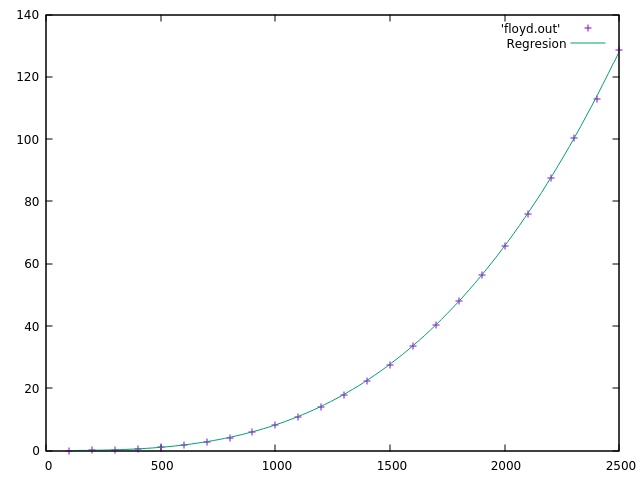
\includegraphics[scale=0.5]{hibrida_floyd.png}
\end{figure}
\end{frame}

\subsubsection{Algoritmos con eficiencia $O(n \cdot log(n))$}

\begin{frame}[fragile]{Algoritmo mergesort}
\begin{figure}[H]
\centering
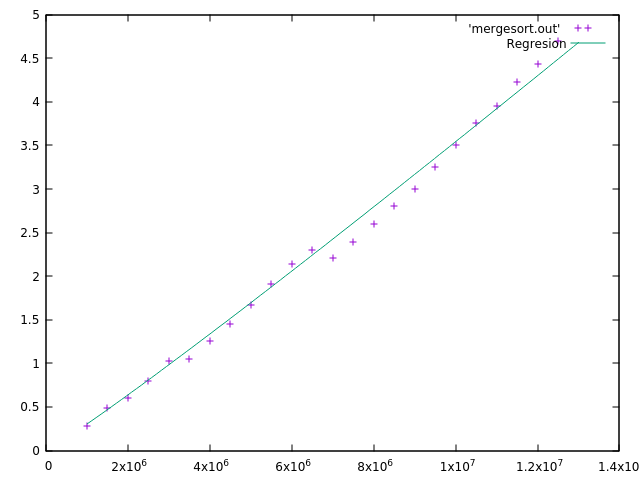
\includegraphics[scale=0.5]{hibrida_mergesort.png}
\end{figure}
\end{frame}

\begin{frame}[fragile]{Algoritmo quicksort}
\begin{figure}[H]
\centering
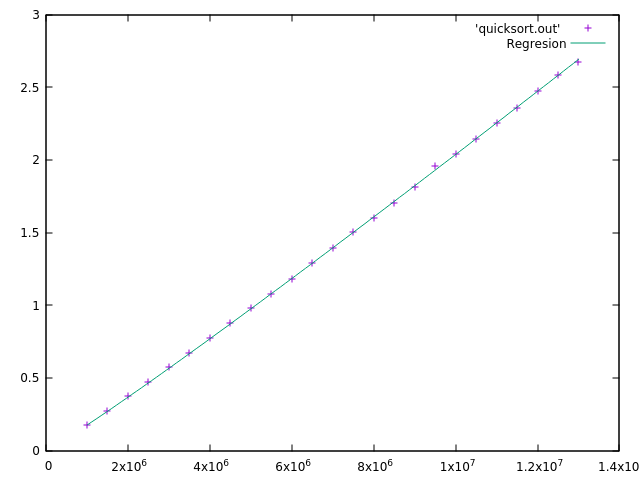
\includegraphics[scale=0.5]{hibrida_quicksort.png}
\end{figure}
\end{frame}

\begin{frame}[fragile]{Algoritmo heapsort}
\begin{figure}[H]
\centering
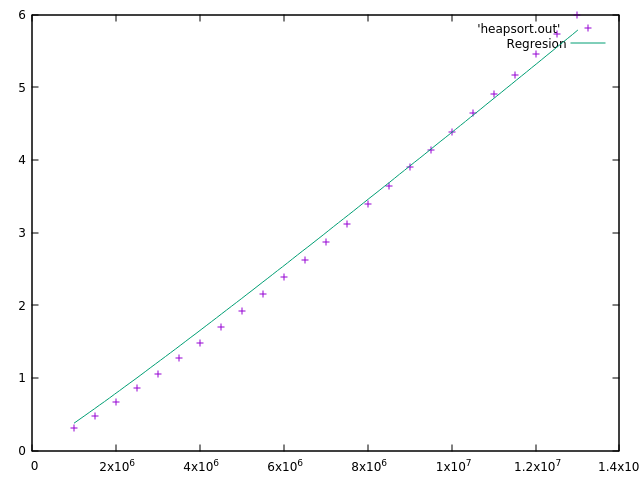
\includegraphics[scale=0.5]{hibrida_heapsort.png}
\end{figure}
\end{frame}

\subsubsection{Algoritmo con eficiencia $O(2^n)$}

\begin{frame}[fragile]{Algoritmo Hanoi}
\begin{figure}[H]
\centering
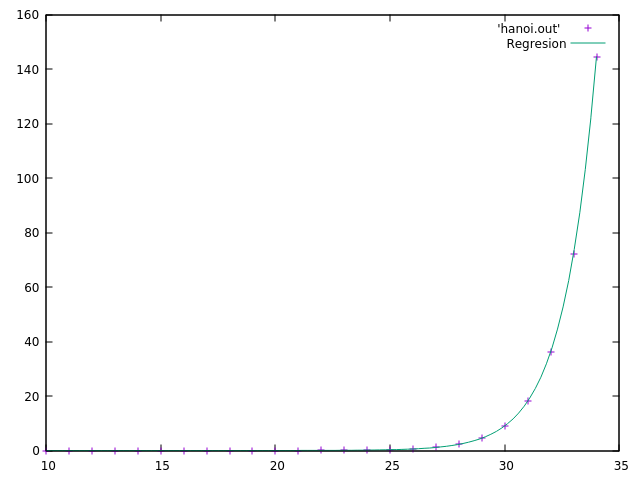
\includegraphics[scale=0.5]{hibrida_hanoi.png}
\end{figure}
\end{frame}

\subsection{Ajuste erróneo}

\begin{frame}[fragile]{Ajuste erróneo}
\begin{figure}[H]
\centering
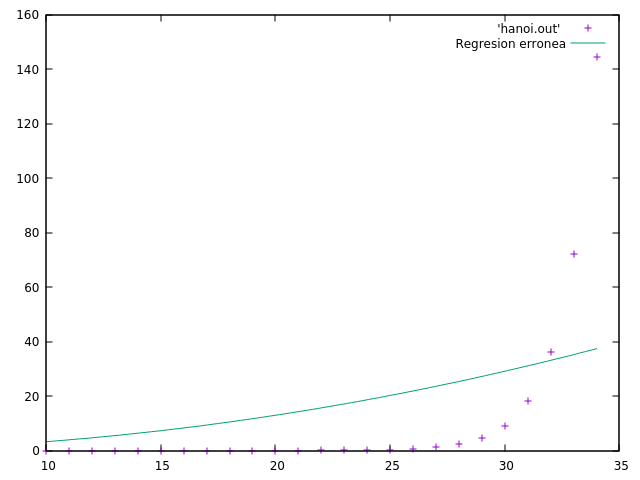
\includegraphics[scale=0.5]{ajuste_erroneo.png}
\end{figure}
\end{frame}

\section*{Fin de la presentación}
\begin{frame}{Fin}
\begin{center}
\huge{Fin de la presentación}
\end{center}
\end{frame}


\end{document}


